\chapter{Feinkörnige Nebenläufigkeit}
Problem: Bei einem hohen Grad an Nebenläufigkeit wird der Zugriff auf das gemeinsame Objekt zum Flaschenhals. Die Threads können nur nacheinander zugreifen.\\
Abhilfe: 4 Techniken.
\begin{enumerate}
	\item \textbf{Feinkörnige Synchronisation:} Statt das Objekt zu sperren, werden nur die betroffenen Komponenten gesperrt. Nur wenn zwei Threads auf dieselbe Komponente zugreifen wollen, muss einer warten.
	\item \textbf{Optimistische Synchronisation:} Während der Suche nach einer bestimmten Komponente des Objekts werden keine Sperren erworben. Sobald die Komponente gefunden wurde, diese Komponente sperren und überprüfen, ob sich der Kontext inzwischen verändert hat.
	\item \textbf{Faule Synchronisation:} Löschen einer Komponente wird in zwei Phasen durchgeführt:
	\begin{enumerate}
		\item Als gelöscht markieren, z.B. durch Setzen eines gewissen Bits ("`logisches Löschen"').
		\item Aus der Datenstruktur aushängen ("`physikalisches Löschen"').
	\end{enumerate}
	\item \textbf{Nicht-blockierende Synchronisation:} Statt Sperren werden atomare Operationen verwendet.
\end{enumerate}

\section[Mengen mit verketteten Listen]{Beispiel: Mengen implementiert durch verkettete Listen}
Mengen-Schnittstelle:
\begin{lstlisting}
Typ Set<T>
Methoden
    add(T x) // x zu Menge this hinzufuegen
    remove(T x) // x aus Menge this entfernen
    containes(T x) // Wahrheitswert von "this enthaelt x"
\end{lstlisting}
Implementierung von Mengen durch verkettete Listen mit Wächtern, sortiert nach Streuwert.\\
\\
Listenelement (Typ Node<T>) habe folgende Attribute:\\
\begin{description}
	\item[T item] das Element der Menge
	\item[int key] der Streuwert des Elements
	\item[Node<T> next] Zeiger auf das nächste Element
\end{description}

\begin{description}
	\item[Wächter (engl. Sentinel)] "`künstliches"' Listenelement, das Anfang oder Ende der Liste markiert.
\end{description}

Beispiel:
\begin{figure}[H]
	\begin{center}
		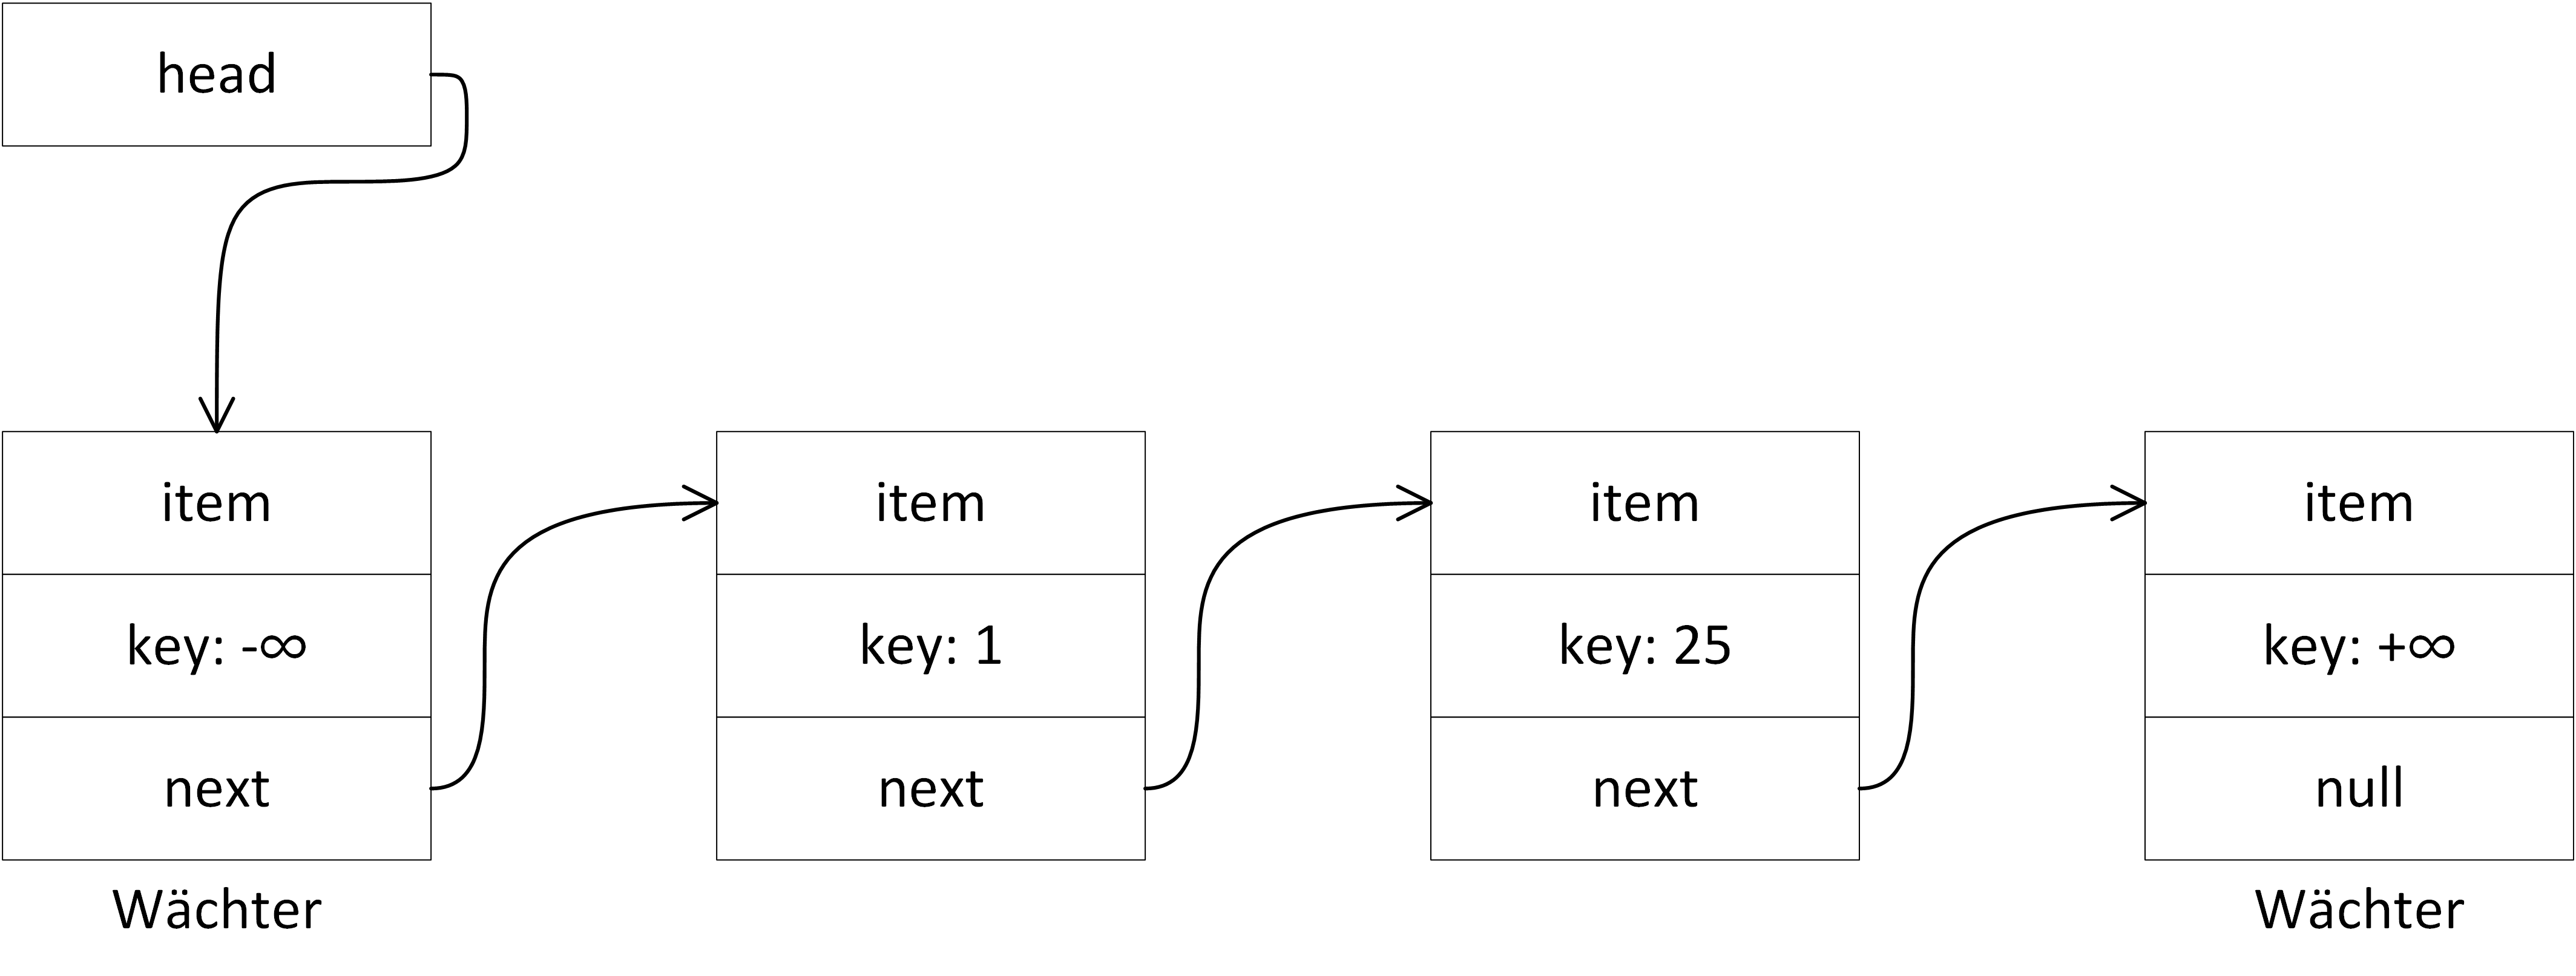
\includegraphics[width=\textwidth]{res/linkedlist}
		\caption{Visualisierung einer LinkedList.}
		\label{pic:linkedlist}
	\end{center}
\end{figure} 
Die Streuwerte sind sortiert: $ -\infty \leq 1 \leq 25 \leq +\infty $.\\
\\
Klasse List<T> mit Attribut head vom Typ Node<T>.\\
Invariante: Wächter werden weder hinzugefügt noch gelöscht. Die Listenelemente sind nach Streuwert sortiert.

\section{Implementierung mit Feinkörniger Synchronisation}
In Java:
\begin{lstlisting}
class List<T> {
	...
	public boolean add(T x) {
		int k = x.hashCode(); // Streuwert
		Node<T> pred, curr;
		try {
			pred = this.head;
			curr = pred.next;
			pred.lock(); // Assume implementation
			curr.lock();
			while (curr.key < k) {
				pred.unlock();
				pred = curr;
				curr = pred.next;
				curr.lock();
			}
			if (curr.key != k) {
				Node<T> node = new Node<>(x);
				node.next = curr;
				pred.next = node;
			}
		} finally {
			curr.unlock();
			pred.unlock();
		}
	}
}
\end{lstlisting}

Methoden remove und contains ähnlich.\\
\\
Eine Sperre genügt nicht. Beispiel dazu:
\begin{figure}[H]
	\begin{center}
		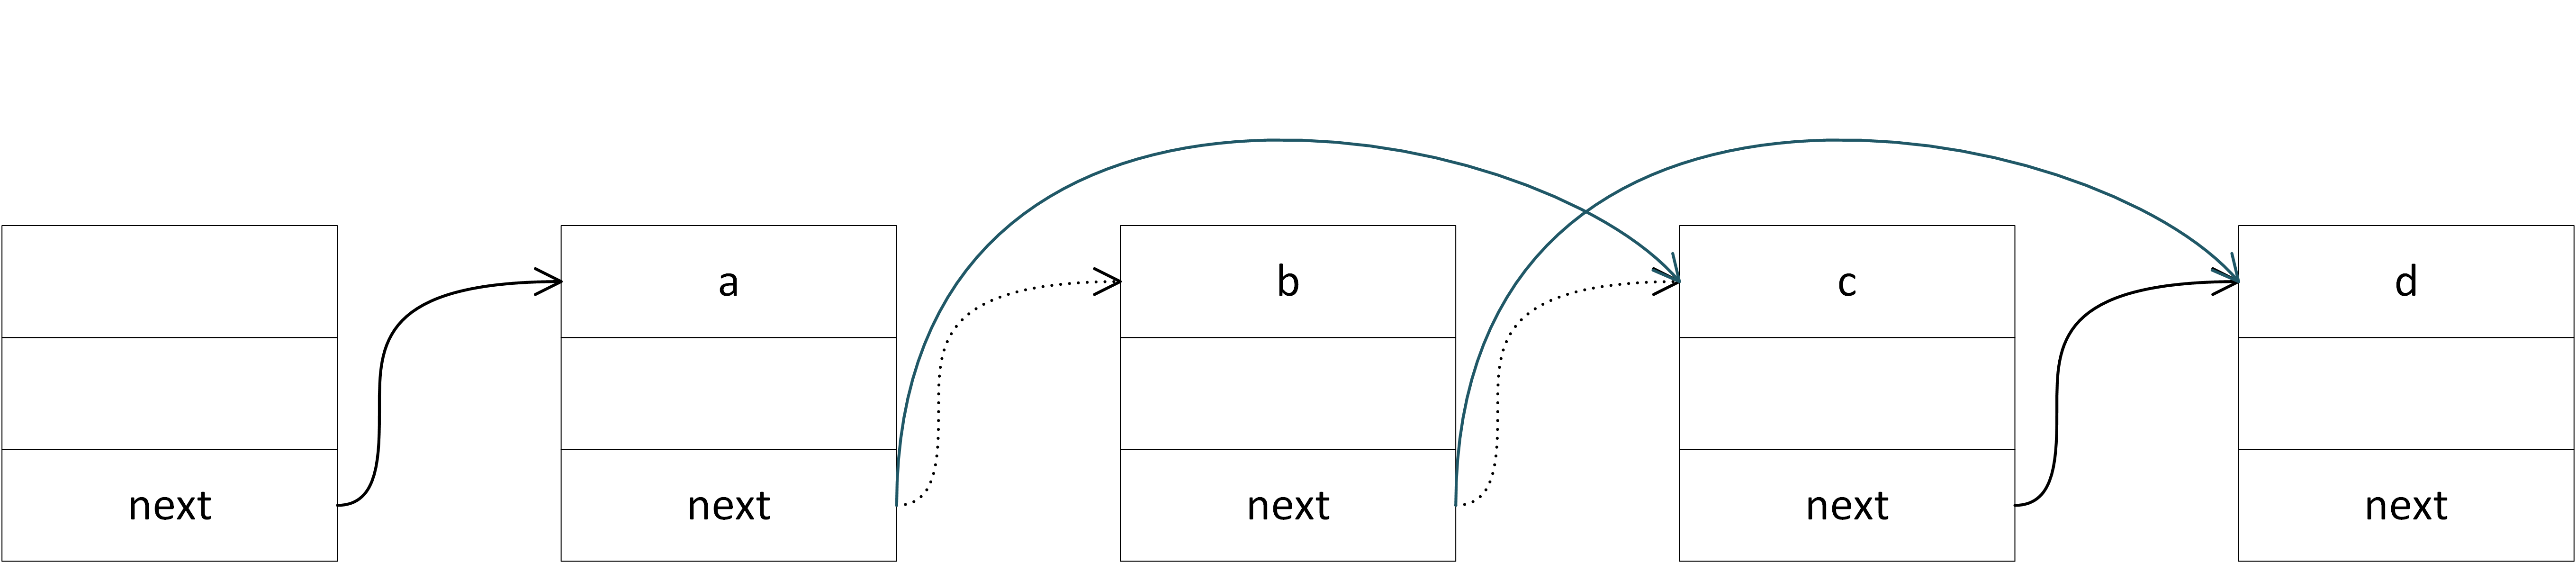
\includegraphics[width=\textwidth]{res/linkedlist_onelock}
		\caption{Visualisierung einer LinkedList.}
		\label{pic:linkedlistonelock}
	\end{center}
\end{figure} 
Thread 1 will b löschen:
\begin{itemize}
	\item Sperre in a erwerben
	\item a.next auf c setzen
\end{itemize}
Thread 2 will c löschen:
\begin{itemize}
	\item Sperre in b erwerben
	\item b.next auf d setzen
\end{itemize}
Wirkung: Nur b wird gelöscht!\\
\\
Um b zu löschen, muss die Sperre in a und in b erworben werden, und entsprechend um c zu löschen, muss die Sperre in b und in c erworben werden. $\Rightarrow$ Konflikt!

\pagebreak

\section{Implementierung mit optimistischer Synchronisation}

In Java:
\begin{lstlisting}
class OptList<T> {
	...
	public boolean add(T x) {
		int k = x.hashCode();
		Node<T> pred, curr;
		boolean done = false;
		while (!done) {
			pred = this.head;
			curr = pred.next;
			while (curr.key < k) {
				pred = curr;
				curr = pred.next;
			}
			try {
				pred.lock();
				curr.lock();
				if (this.validate(pred, curr)) {
					if (curr.key != k) {
						Node<T> node = new Node<>(x);
						node.next = curr;
						pred.next = node;
					}
					done = true;
				}
			} finally {
				curr.unlock();
				pred.unlock();
			}
		}
	}
	
	private boolean validate(Node<T> pred, Node<T> curr) {
		Node<T> node = this.head;
		while (node.key < pred.key) {
			node = node.next;
		}
		return node == pred && curr = node.next;
	}
}
\end{lstlisting}
Diskussion: Optimistisches Synchronisation lohnt sich, wenn zweimaliges Durchlaufen der Liste billiger ist als einmaliges Durchlaufen mit Setzen von Sperren. Belegen und Freigeben sind aufwendig.

\section{Implementierung mit fauler Synchronisation}
Listenelemente bekommen ein neues Attribut: \emph{marked} drückt aus, dass es zum Löschen markiert wurde.\\
\\
Neue Version von validate:
\begin{lstlisting}
private boolean validate(Node<T> pred, Node<T> curr) {
	return !pred.marked && !curr.marked && pred.next == curr;
}
\end{lstlisting}
Löschen:
\begin{lstlisting}
public boolean remove(T item) {
	int k = item.hashCode();
	boolean done = false;
	boolean erg = false;
	while (!done) {
		Node<T> pred = this.head;
		Node<T> curr = pred.next;
		while (curr.key < k) {
			pred = curr;
			curr = pred.next;
		}
		pred.lock();
		try {
			curr.lock();
			try { // falls erste Sperre geht, aber zweite nicht
				if (validate(pred, curr)) {
					if (curr.key == j) {
						curr.marked = true;
						pred.next = curr.next;
						erg = true;
					}
					done = true;
				}
			} finally {
				curr.unlock();
			}
		} finally {
			pred.unlock();
		}
	}
	return erg;
}
\end{lstlisting}
Contains:
\begin{lstlisting}
public boolean contains(T item) {
	int k = item.hashCode();
	Node<T> curr = this.head;
	while (curr.key < k) {
		curr = curr.next;
	}
	return curr.key == key && !curr.marked;
}
\end{lstlisting}